%% LaTeX Beamer presentation template (requires beamer package)
%% see http://bitbucket.org/rivanvx/beamer/wiki/Home
%% idea contributed by H. Turgut Uyar
%% template based on a template by Till Tantau
%% this template is still evolving - it might differ in future releases!

\documentclass[10pt]{beamer}

\mode<presentation>
{
\usetheme{Malmoe}

\setbeamercovered{transparent}
}


\addtobeamertemplate{navigation symbols}{}{%
\usebeamerfont{footline}%
\usebeamercolor[fg]{footline}%
\hspace{1em}%
\insertframenumber/\inserttotalframenumber
}

\usepackage[brazil]{babel}
\usepackage[utf8]{inputenc}
\usepackage{listings}

% font definitions, try \usepackage{ae} instead of the following
% three lines if you don't like this look
\usepackage{mathptmx}
\usepackage[scaled=.90]{helvet}
\usepackage{courier}
\usepackage{url}


\usepackage[T1]{fontenc}

\title{Comparação do número de acessos à memória e TLB \textit{misses} com
páginas de 4KB ou 4MB}

%\subtitle{}

% - Use the \inst{?} command only if the authors have different
%   affiliation.
%\author{F.~Author\inst{1} \and S.~Another\inst{2}}
\author{Gustavo Ciotto Pinton}

% - Use the \inst command only if there are several affiliations.
% - Keep it simple, no one is interested in your street address.
\institute
{

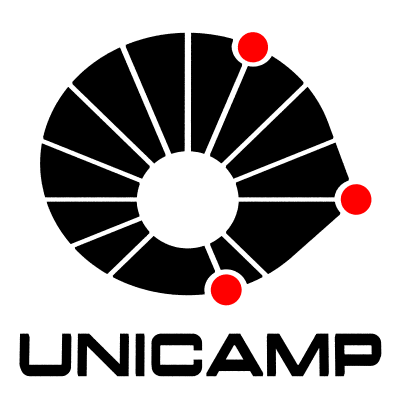
\includegraphics[scale=0.12]{logo} \\
\vspace{16pt}
Universidade Estadual de Campinas - UNICAMP\\
MO601B - Arquitetura de Computadores}

\date{21 de Outubro de 2016}



% If you have a file called "university-logo-filename.xxx", where xxx
% is a graphic format that can be processed by latex or pdflatex,
% resp., then you can add a logo as follows:

% \pgfdeclareimage[height=0.5cm]{university-logo}{university-logo-filename}
% \logo{\pgfuseimage{university-logo}}



% Delete this, if you do not want the table of contents to pop up at
% the beginning of each subsection:
\AtBeginSubsection[]
{
\begin{frame}<beamer>
\frametitle{Outline}
\tableofcontents[currentsection,currentsubsection]
\end{frame}
}

% If you wish to uncover everything in a step-wise fashion, uncomment
% the following command:

%\beamerdefaultoverlayspecification{<+->}

\begin{document}

\begin{frame}

\titlepage
\end{frame}

\section{Contagem de instruções dos benchmarks}


\begin{frame}
\frametitle{Contagem de acessos à memória}
\framesubtitle{Escolha dos \textit{caches}}

\begin{itemize}
  \item TLBs de dados e instruções: 512 entradas e \textit{fully associatives}.
  2 pares de \textit{TLB instruções} + \textit{TLB dados}.
  
  \item O primeiro nível L1 contém dois caches dedicados para instruções e
  dados, separadamente, com 64KB cada e 32-way associative.
   
  \item L2 é unificado para instruções e dados, possuindo 256KB
  e 8-way associative.
  
  \item Cache L3, possui 4MB, sendo 16-way associative.
  
  \vspace{12pt}
  
  \item \textit{Pinballs}:  100M \textit{warmup}, regiões de 30M e
  max(K) = 10.

  \vspace{12pt}
  
  \item Dados coletados por um \textit{script python}. 
\end{itemize}
\end{frame}

\begin{frame}
\frametitle{Contagem de acessos à memória}
\framesubtitle{Páginas de 4KB}

\begin{columns}

\column{0.58\textwidth}
\begin{figure}[h!]
\centering
\centering

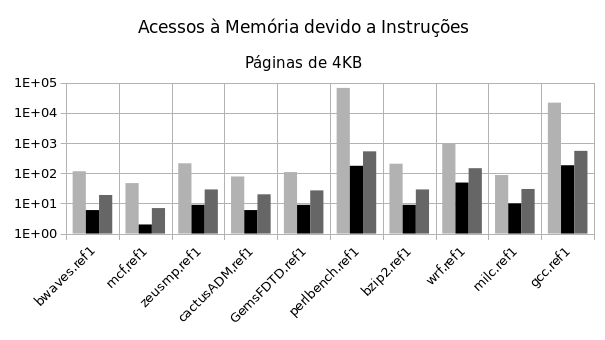
\includegraphics[width=0.9\linewidth]{inst_4KBs}
\caption{Acessos à memória, TLB \textit{misses} e acessos à tabela de páginas
devido a instruções.}
\end{figure}

\column{0.58\textwidth}
\begin{figure}[h!]
\centering
\centering

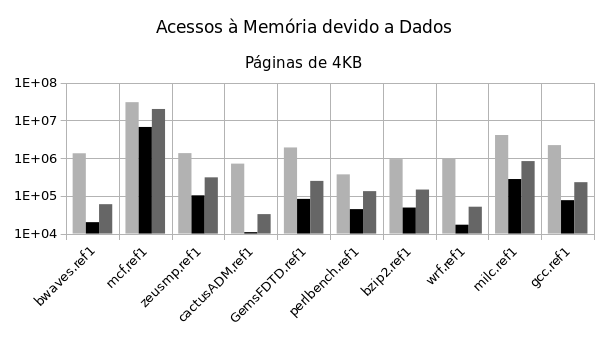
\includegraphics[width=0.9\linewidth]{data_4KBs}
\caption{Acessos à memória, TLB \textit{misses} e acessos à tabela de páginas
devido a dados.}
\end{figure}
\end{columns}

\end{frame}

\begin{frame}
\frametitle{Contagem de acessos à memória}
\framesubtitle{Páginas de 4MB}

\begin{columns}

\column{0.58\textwidth}
\begin{figure}[h!]
\centering
\centering

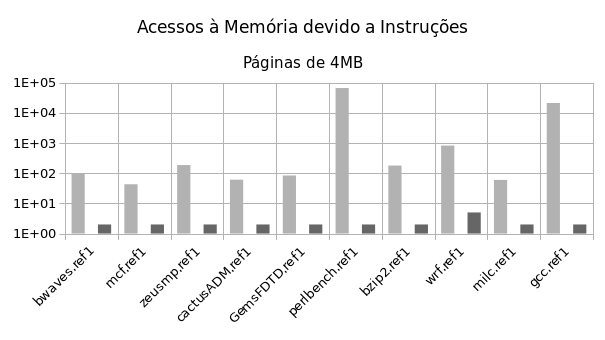
\includegraphics[width=0.9\linewidth]{inst_4MBs}
\caption{Acessos à memória, TLB \textit{misses} e acessos à tabela de páginas
devido a instruções.}
\end{figure}

\column{0.58\textwidth}
\begin{figure}[h!]
\centering
\centering

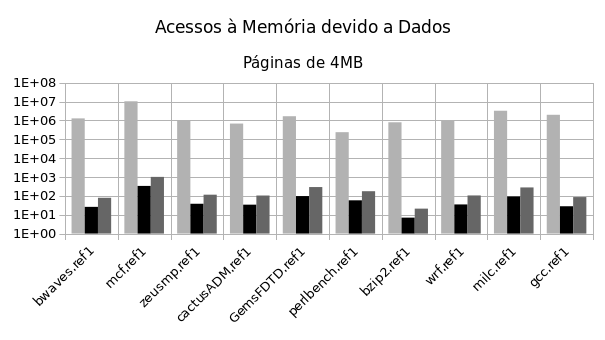
\includegraphics[width=0.9\linewidth]{data_4MBs}
\caption{Acessos à memória, TLB \textit{misses} e acessos à tabela de páginas
devido a dados.}
\end{figure}
\end{columns}

\end{frame}

\begin{frame}
\frametitle{Contagem de acessos à memória}
\framesubtitle{\textit{Toy benchmark}}

\begin{itemize}
\item 2 vetores:
\begin{itemize}
  \item double*  double\_pointer\_array [\(512 * PAGE\_SIZE\)]
  \item int*  int\_pointer\_array [\(512 * PAGE\_SIZE\)]
\end{itemize}
\item Para cada item pertencente a este vetor: malloc (\(1*PAGE\_SIZE\)).
\vspace{12pt}
\item Acessos sequenciais e 15000 acessos aleatórios.
\vspace{12pt}
\item Espera-se desempenho ruim da TLB para páginas de 4KB e bom para
4MB.
\end{itemize}

\end{frame}

\begin{frame}
\frametitle{Contagem de acessos à memória}
\framesubtitle{\textit{Toy benchmark}}

\begin{columns}

\column{0.50\textwidth}
\begin{figure}[h!]
\centering 

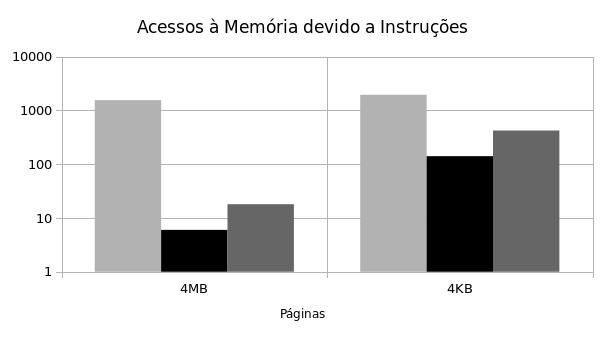
\includegraphics[width=0.9\linewidth]{toy_inst}
\caption{Acessos à memória devido a instruções.}
\end{figure}

\column{0.50\textwidth}
\begin{figure}[h!]
\centering
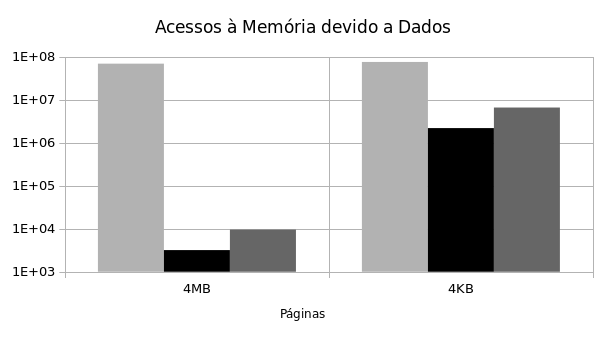
\includegraphics[width=0.9\linewidth]{toy_data}
\caption{Acessos à memória devido a dados.}
\end{figure}
\end{columns}
 
\end{frame}

\begin{frame}
\frametitle{Conclusões}
\framesubtitle{Resultados}

\begin{itemize}
    \item Páginas de 4KB: acessos adicionais causados por \textit{misses} na TLB
    de instruções ou dados são uma fração importante do número total.

  \vspace{12pt}

  \item Páginas de 4MB: o número de \textit{misses} na TLB de instruções é
  praticamente nulo. Os acessos à memória são gerados exclusivamente por
  \textit{misses} em L3. 
  
  \vspace{12pt}

  \item Páginas de 4MB : acessos à tabela de
  páginas devido a dados são inferiores àqueles de 4KB, mas ainda representam
  uma fração considerável. 
\end{itemize}

\end{frame}


\begin{frame}
\frametitle{Referências}

\begin{itemize}
  \item Henning, J. L. (2007). Spec cpu2006 memory footprint. \textit{ACM
  SIGARCH Computer Architecture News}, 35;
  \vspace{14pt}
  \item SniperSim (2008). Pinballs, disponível em
  \url{http://snipersim.org/w/Pinballs}.
  \item Intel® 64 and IA-32 Architectures
Software Developer’s Manual, disponível em \url{http://intel.ly/KqEL7c}.
\end{itemize}

\end{frame}

\end{document}
